\section{Need For Speed Hot Pursuit}

\begin{figure}[htbp]
\begin{center}
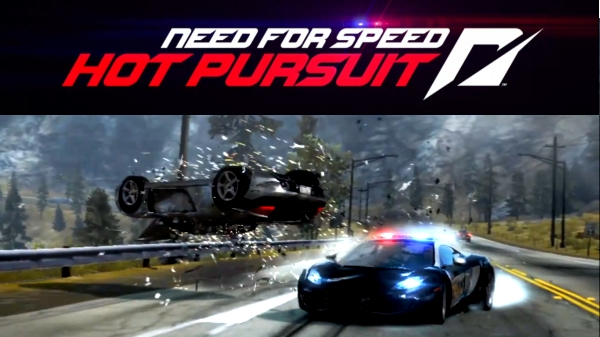
\includegraphics[width=.60\textwidth]{./imagenes/NeedForSpeedHotPursuit.jpg}
\caption{Need For Speed Hot Pursuit}
\label{Need For Speed Hot Pursuit}
\end{center}
\end{figure}

Need For Speed Hot Pursuit\footnote{\url{http://www.needforspeed.com/es_ES/hot-pursuit}}es el nombre de la decimocuarta entrega de la saga Need for Speed. Es un juego de carreras de 2010 desarrollado por Criterion Games y publicado por Electronic Arts para PlayStation 3, Xbox 360, Microsoft Windows, Wii y iPhone.6 7 También hay una versión para Wii, desarrollada por Exient. El juego ha sido descrito como una "revolucionaria" adición de la saga Need for Speed y fue lanzado enNorteamérica el 16 de noviembre de 2010, y en Europa el 18 de noviembre.

El juego está inspirado en Need for Speed: Hot Pursuit original, basado a su vez en las persecuciones de alta velocidad con autos exóticos. Como se ha visto en juegos anteriores, en Hot Pursuit se tiene la oportunidad de ser un policía o un piloto huyendo de la justicia. Hot Pursuit se centra en un lugar ficticio llamado Seacrest County, lugar muy abierto que permite al jugador correr durante varios kilómetros.

\subsubsection{¿Por qué es uno de mis juegos favoritos?}
\begin{itemize}
\item[Esteban Muñoz]Este consiste en que el jugador tiene que ganar la carrera escapando de la      policía, o jugar como policía e intentar dar caza y arrestar a los pilotos que infringieran los límites de velocidad. Muchos de los coches y circuitos no están disponibles al comenzar el juego. El objetivo es desbloquearlos al ganar carreras.El juego disponía de coches exóticos como el Lamborghini Diablo SV, Mercedes-Benz CLK GTR o el Jaguar XJR-15,coches especiales (el phanton y el titan) cuyas características son de estabilidad y velocidad extrema,los cuales aparecen en el juego por medio de claves especiales escritas en el user name y un coche inventado por los creadores (siendo este el de mejor características) llamado "El Niño" y en el modo hot pursuit tiene como extra un helicóptero de policía. Además incluye pistas como una en la que se pasa debajo de un túnel de cristal, en una especie de lago o una ciudad. Pasando por cañones, por zonas rurales, e inclusive carreteras urbanas. Otra característica era que el trazado podía ser de noche o de día y con lluvia o nieve.
\end{itemize}
